% (c) 2012 Tiziana Manca - tmanca@libero.it
% (c) 2012 -2014 Dimitrios Vrettos - d.vrettos@gmail.com
% (c) 2014 Daniele Zambelli - daniele.zambelli@gmail.com

\chapter{Statistica descrittiva bivariata}

\section{Indagine statistica}
\label{sec:A_indagine}

Il termine statistica significa \emph{scienza dello stato}. Questo termine 
venne usato per la prima volta nel~$XVI$ secolo
per indicare lo studio dei dati utili al governo degli stati 
prevalentemente relativi a fenomeni di carattere demografico (nascite, 
morti, etc).
Negli anni, la statistica si è estesa ai campi più disparati: fisica, 
psicologia, ricerca di mercato, indici di gradimento, sondaggi, 
meteorologia\ldots
È nata essenzialmente con lo scopo di descrivere i fenomeni (statistica 
descrittiva), successivamente è divenuta uno strumento utile
anche per fare previsioni (statistica inferenziale). In grandi linee si può 
definire come la scienza che si occupa della raccolta e dell'analisi dei 
dati relativi
ad un certo gruppo di persone, animali o oggetti al fine di descrivere in 
maniera sintetica un fenomeno che li riguarda e fare eventualmente 
previsioni sul suo andamento futuro.

Ad esempio la statistica cerca di fare previsioni su domande del tipo:
\begin{itemize*}
\item quanta acqua sarà necessaria in Italia fra~3 anni?
\item quanta corrente elettrica sarà necessaria per il fabbisogno nazionale 
fra~5 anni?
\item quale sarà il tasso di disoccupazione nazionale fra~1 anno?
\end{itemize*}

\begin{definizione}
L'insieme di elementi oggetto dell'indagine statistica è detta 
\emph{popolazione} o universo, mentre ciascun elemento della popolazione è 
detto \emph{unità statistica}.
\end{definizione}

Sono esempi di \emph{popolazione statistica} gli abitanti di una città in 
un certo anno, i prezzi di un determinato bene, le temperature massime 
registrate
in una giornata in un particolare luogo, i ciclomotori circolanti in 
Italia, gli alunni di una scuola.

\begin{definizione}
Per ogni unità statistica si possono studiare una o più caratteristiche ed 
ognuna di tali caratteristiche costituisce un \emph{carattere} della 
popolazione oggetto
di indagine. I caratteri possono essere di tipo qualitativo o quantitativo.
Si definisce \emph{modalità} del carattere indagato ciascuno dei diversi 
modi in cui esso può presentarsi.
\end{definizione}

Sono esempi di \emph{carattere qualitativo} il colore degli occhi, il 
colore dei capelli, il tipo di scuola frequentato, il gradimento di un 
certo programma televisivo.
Le modalità di un carattere qualitativo sono espresse mediante nomi o 
aggettivi.
I caratteri qualitativi sono a loro volta suddivisi in \emph{ordinabili} 
(il tipo di scuola frequentato è ordinabile a partire dalla scuola 
dell'infanzia fino alla laurea,
il gradimento di un programma televisivo è ordinabile a partire dalla 
completa mancanza di gradimento fino al gradimento massimo) e \emph{non 
ordinabili} o sconnessi
(colore degli occhi, colore dei capelli).

Sono invece \emph{caratteri quantitativi} l'età, l'altezza, il numero di 
auto prodotte da una fabbrica. Le modalità di un carattere quantitativo 
sono espresse mediante numeri.
I caratteri quantitativi possono invece essere di tipo \emph{discreto}, 
quando assumono solo valori puntuali, oppure di tipo \emph{continuo}, 
quando possono assumere
tutti gli infiniti valori compresi in un determinato intervallo. Sono 
esempi di caratteri quantitativi discreti il numero di figli in una 
famiglia,
i pezzi prodotti in una catena di montaggio; sono esempi di caratteri 
continui l'altezza di una persona, il peso di una persona, la lunghezza di 
un fiume.

L'indagine statistica può riguardare l'intera popolazione (in tal caso si 
parla di \emph{censimento}) oppure solo una sua parte (in tal caso si parla 
di indagine a campione).
Supponiamo di voler effettuare un'indagine sulle persone che fumano in 
Italia. Il fenomeno collettivo in esame è il fumo, la popolazione di 
riferimento
è costituita dalla popolazione italiana in età adulta, l'unità statistica è 
rappresentata da ogni cittadino oggetto dell'indagine, i caratteri oggetto
dell'indagine possono essere ``fumatore / non fumatore'', ``numero di 
sigarette fumate'', che cosa si fuma: pipa, sigaro, sigaretta. Data 
l'elevata numerosità
della popolazione di riferimento la tipologia di indagine preferibile è 
quella a campione.

A sua volta, l'indagine a campione può essere effettuata su un 
\emph{campione casuale}, quando si scelgono a caso i campioni all'interno 
della popolazione o
su un \emph{campione stratificato}, quando si suddivide la popolazione in 
classi o strati senza specifici criteri e per ogni strato si prende a caso 
un campione.

% \ovalbox{\risolvi \ref{ese:A.1}}

\section{Fasi di un'indagine statistica}
\label{sec:A_fasi}

\begin{definizione}
Dato un carattere oggetto di rilevazione, si definisce \emph{frequenza} il 
numero delle unità statistiche su cui una sua modalità si presenta.
\end{definizione}
Affinché un'indagine statistica sia rigorosa è necessario che sia 
strutturata secondo le seguenti fasi:

\begin{enumeratea}
\item Studio del problema e impostazione dell'indagine statistica.
Si individua in maniera precisa lo scopo della ricerca, il fenomeno sul 
quale indagare, la popolazione statistica di riferimento,
le singole unità statistiche ed il carattere, o caratteri, oggetto di 
indagine.
\item Rilevazione dei dati statistici.
La rilevazione non è altro che la raccolta dei dati statistici riguardanti 
ogni elemento della popolazione e relativi al fenomeno che si vuole 
analizzare.
La rilevazione può avvenire secondo diverse modalità:
\begin{description}
\item [rilevazione diretta o globale:] viene eseguita direttamente su tutte 
le unità statistiche che formano la popolazione;
\item [rilevazione indiretta o parziale:] eseguita solo su una parte della 
popolazione. Si deve scegliere in tal caso un sottoinsieme della 
popolazione,
detto campione che deve essere rappresentativo della popolazione di 
riferimento.
\end{description}
\item Spoglio delle schede e tabulazione.
Contemporaneamente o successivamente al rilevamento, i dati raccolti 
vengono ordinati, suddivisi in classi omogenee e riassunti tramite tabelle 
dette \emph{tabelle statistiche}.
\item Rappresentazione dei dati statistici.
La rappresentazione può avvenire attraverso diversi tipi di grafico:
\begin{description}
\item [diagramma cartesiano:] rappresentazione nel piano cartesiano dei 
valori della variabile sull'asse orizzontale e delle relative frequenze 
sull'asse verticale;
\item [ideogramma:]si rappresenta un certo numero di dati con un simbolo;
\item [diagramma a nastri o a bastoni:]grafico composto da segmenti o barre 
(orizzontali o verticali) proporzionali alle frequenze;
\item [areogramma:]grafico a forma di cerchio composto da settori circolari 
con aree direttamente proporzionali alle frequenze;
\item [istogramma:] grafico composto da rettangoli aventi area 
proporzionale alla frequenza.
\end{description}
\item Elaborazione dei dati.
Vengono elaborati i dati tabulati al fine di costruire opportuni indici di 
sintesi.
\item Interpretazione dei risultati.
Attraverso i grafici e gli indici è possibile descrivere le caratteristiche 
peculiari del fenomeno analizzato.
\end{enumeratea}
Analizziamo in dettaglio le singole fasi.

\subsection{Spoglio delle schede e tabulazione}
Dopo aver raccolto i dati per ciascuna modalità del carattere o per 
ciascuna classe individuata si deve determinare:

\begin{itemize*}
\item la \emph{frequenza assoluta}, cioè il numero di volte con cui si 
presenta una modalità del carattere indagato;
\item la \emph{frequenza relativa}, cioè il rapporto tra la frequenza 
assoluta e il numero totale dei casi presi in esame;
\item la \emph{frequenza percentuale}, cioè la frequenza relativa 
moltiplicata per~100.
\end{itemize*}
Si compila poi una tabella di frequenza che sintetizza la raccolta dei 
dati, come nell'esempio seguente.

% \begin{exrig}

 \begin{esempio}
Misurando l'altezza di un gruppo di cani di razza pastore italiano si sono 
ottenute le seguenti misure in~$\unit{cm}$:

\begin{center}
 \begin{tabular}{ccccccccccccc}
57,1 & 60,8 & 60,7 & 56,2 & 59,5 & 62,4 & 56,1 & 61,2 & 54,5 & 64,5 & 57,5 
& 58,3 & 55,2\\
58,7 & 57,2 & 56,1 & 58,9 & 57,7 & 53,2 & 59,2 & 58,9 & 54,5 & 55,3 & 62,1 
& 59,0 & 58,3\\
61,3 & 60,1 & 56,4 & 60,2 & 61,7 & 57,3 & 58,3 & 59,5 & 62,6 & 59,4 & 58,3 
& 59,4 & 59,4\\
59,3 & 57,6 & 60,0 & 60,7 & 56,7 & 61,1 & 59,8 & 55,3 & 63,9 & 58,0 & 55,2 
& 54,9 & 53,8\\
 \end{tabular}
\end{center}

Il carattere indagato nella popolazione cani pastore italiano è di tipo 
quantitativo continuo; con questo tipo di dati è praticamente impossibile
calcolare le frequenze se le altezze non si raggruppano in classi.

Vediamo come procedere: osservando i dati ottenuti si nota che il valore 
minore è~$53,8$ mentre il valore maggiore è~$64,7$. Possiamo allora 
suddividere
i dati in gruppi partendo da~$53,0 \unit{cm}$ fino a~$65,0 \unit{cm}$. Si 
potrebbero allora formare classi di ampiezza~$1 \unit{cm}$.
Si ottiene la seguente tabella:

\begin{tabularx}{.9\textwidth}{*{2}{lXX}}
\toprule
Classe ($\unit{cm}$) & Frequenza assoluta & Frequenza percent. &Classe 
($\unit{cm}$) & Frequenza assoluta & Frequenza percent. \\
\midrule
53,0-53,9 & 2 & $3,85\%$ & 59,0-59,9 & 9 & $17,31\%$\\
54,0-54,9 & 3 & $5,77\%$ & 60,0-60,9 & 6 & $11,54\%$\\
55,0-55,9 & 4 & $7,69\%$ & 61,0-61,9 & 4 & $7,69\%$\\
56,0-56,9 & 5 & $9,61\%$ & 62,0-62,9 & 3 & $5,77\%$\\
57,0-57,9 & 6 & $11,54\%$ & 63,0-63,9 & 1 & $1,92\%$\\
58,0-58,9 & 8 & $15,38\%$ & 64,0-64,9 & 1 & $1,92\%$\\
\midrule
Totale & 52 & &&&\\
\bottomrule
\end{tabularx}
\end{esempio}
% \end{exrig}


Riassumendo
\begin{center}
 % (c) 2012 Dimitrios Vrettos - d.vrettos@gmail.com
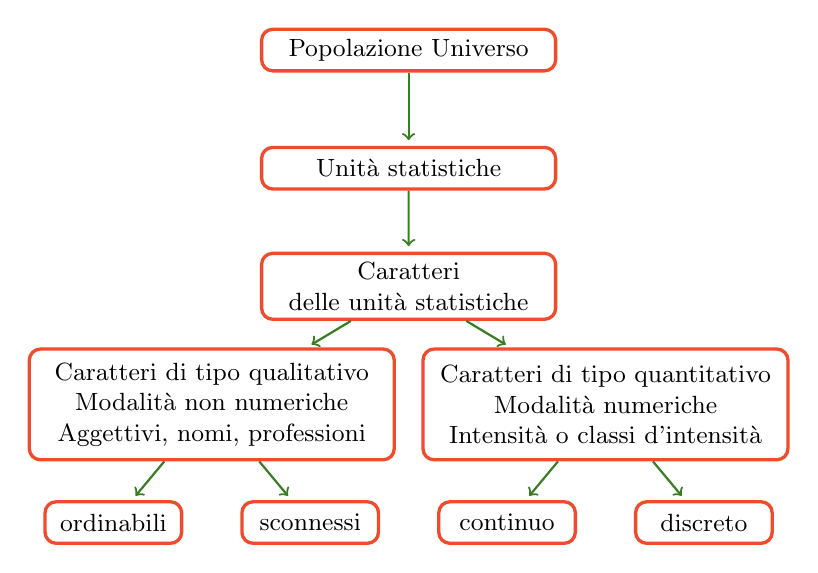
\begin{tikzpicture}[font=\small,
  punto/.style={%
    draw=RedOrange, 
    rectangle, 
    fill=white,
    very thick, 
    rounded corners,
    text centered,
    text width=35mm,
    minimum height=1.5em},
  subpunto/.style={%
    draw=RedOrange, 
    rectangle, 
    fill=white,
    very thick, 
    rounded corners,
    text centered,
    text width=44mm,
    minimum height=4em},
  subpunto1/.style={%
    draw=RedOrange, 
    rectangle, 
    fill=white,
    very thick, 
    rounded corners,
    text centered,
    text width=15mm,
    minimum height=1.5em},
  level distance=15mm,
  level 3/.style={sibling distance=50mm},
  level 4/.style={sibling distance=25mm}, 
  edge from parent/.style={draw,->,OliveGreen, thick, shorten >=2pt}]
  
\node [punto] {Popolazione Universo}
  child {node [punto] {Unit\`a statistiche}
    child {node [punto]{Caratteri \\delle unit\`a statistiche}
      child{node [subpunto]{Caratteri di tipo qualitativo \\Modalit\`a non numeriche \\Aggettivi, nomi, professioni}
	child {node [subpunto1]{ordinabili}}
	child {node [subpunto1]{sconnessi}}}
      child {node [subpunto]{Caratteri di tipo quantitativo \\Modalit\`a numeriche \\Intensit\`a o classi d'intensit\`a}
	child {node[subpunto1] {continuo}}
	child {node[subpunto1] {discreto}}}}};
\end{tikzpicture}

\end{center}

% \ovalbox{\risolvii \ref{ese:A.2}, \ref{ese:A.3}, \ref{ese:A.5}, 
% \ref{ese:A.6}, \ref{ese:A.7}, \ref{ese:A.8}, \ref{ese:A.9}}

\subsection{Rappresentazione grafica}

La rappresentazione grafica dei dati statistici facilita notevolmente lo 
studio delle caratteristiche del
fenomeno statistico che si sta esaminando; infatti dopo aver impostato 
l'indagine, raccolto, classificato ed elaborato i dati nelle tabelle,
i dati non sempre si presentano in una forma di facile lettura ed il loro 
significato e la loro interpretazione rimane poco chiara.
Attraverso la rappresentazione grafica, i risultati dell'indagine emergono 
immediatamente, in maniera diretta e sintetica.

La rappresentazione grafica può avvenire utilizzando diversi tipi di 
grafico a seconda delle caratteristiche da
analizzare.

\subsubsection{Diagramma cartesiano}
La rappresentazione grafica attraverso un diagramma cartesiano dà, in modo 
immediato, informazioni sull'andamento globale del fenomeno e viene
utilizzato prevalentemente per la rappresentazione di serie storiche (per 
esempio, per rappresentare il numero di auto prodotte per anno da una 
fabbrica)
oppure quando si hanno due caratteri quantitativi e si vuol analizzare il 
tipo di legame esistente fra di essi.


% \begin{exrig}
 \begin{esempio}

Consideriamo la tabella statistica relativa alla domanda ``quante ore al 
giorno passi al computer?'', posta ad un
campione di~50 ragazzi dai~16 ai~24 anni.

Rappresentiamo la tabella attraverso un diagramma cartesiano costruito 
tracciando due rette perpendicolari, gli assi, quello verticale orientato 
verso
l'alto e quello orizzontale orientato verso destra. Riportiamo sull'asse 
orizzontale il numero di ore e sull'asse verticale il numero di ragazzi e 
determiniamo
i punti aventi come coordinate (numero ore; numero ragazzi).

Il punto~$A$ avrà come coordinate~0 e~4, il punto~$B$ avrà come 
coordinate~1 e~6 e così via. Uniamo poi
i punti con segmenti e otteniamo il diagramma 
cartesiano~(grafico~\ref{gr:A.1}).
Precisamente~$A(0;4)$, $B(1;6)$, $C(2;12)$, $D(3;16)$, $E(4;8)$, $F(5;4)$, 
$G(6;2)$.

\begin{center}
\begin{tabular}{lccccccc}
\toprule
Numero di ore & 0 & 1 &2 & 3 & 4 & 5 & 6\\
Numero di ragazzi & 4 & 6 & 12 & 16 & 8 & 4 & 2 \\
\bottomrule
\end{tabular}
\end{center}
Dal grafico~\ref{gr:A.2} si può notare immediatamente che la maggior parte 
dei ragazzi trascorre dalle~2 alle~3 ore al computer dato che il picco più
alto si ha proprio nei punti~$C$ e~$D$.
Si può notare che, ad esempio, il punto~$X$ di coordinate~$(3.5;12)$, 
appartenente al segmento di congiunzione tra i punti~$D$ ed~$E$,
non ha significato reale, dato che le sue coordinate non sono riportate 
nella tabella statistica del fenomeno da studiare.
\begin{grafico}[t]
\begin{minipage}{0.5\textwidth}
% (c) 2012 Dimitrios Vrettos - d.vrettos@gmail.com
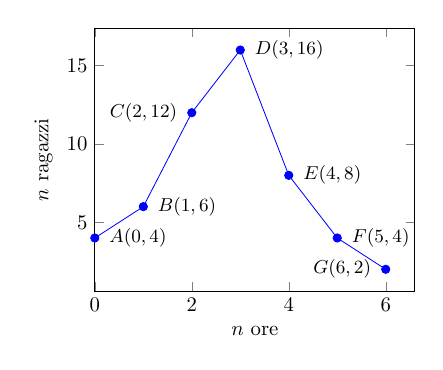
\begin{tikzpicture}[scale=.75]
  \tikzset{
    every pin/.style={pin distance=0,font=\small},
  }

\begin{axis}[xlabel=$n\grado$ ore, ylabel=$n\grado$ ragazzi,xmin=0]
  \addplot[color=blue, mark=*]
    coordinates{
      (0,4) 
      (1,6)
      (2,12)
      (3,16)
      (4,8)
      (5,4)
      (6,2)
      };

  \node[pin=0:{$A(0,4)$}] at (axis cs:0,4) {};
  \node[pin=0:{$B(1,6)$}] at (axis cs:1,6) {};
  \node[pin=180:{$C(2,12)$}] at (axis cs:2,12) {};
  \node[pin=0:{$D(3,16)$}] at (axis cs:3,16) {};
  \node[pin=0:{$E(4,8)$}] at (axis cs:4,8) {};
  \node[pin=0:{$F(5,4)$}] at (axis cs:5,4) {};
   \node[pin=180:{$G(6,2)$}] at (axis cs:6,2) {};
\end {axis}
\end{tikzpicture}

\caption{Esempio~24.4}\label{gr:A.1}
\end{minipage}\hfill
\begin{minipage}{0.5\textwidth}
% (c) 2012 Dimitrios Vrettos - d.vrettos@gmail.com
\begin{tikzpicture}[scale=.75]
  \tikzset{
    every pin/.style={pin distance=0,font=\small},
  }

  \begin{axis}[xlabel=$n\grado$ ore, ylabel=$n\grado$ ragazzi,xmin=0]
    \addplot[only marks, color=blue, mark=*]
      coordinates{
	(0,4) 
	(1,6)
	(2,12)
	(5,4)
	(6,2)
      };
 \addplot[color=grigio70, mark=*]
      coordinates{
	(0,4)
	(1,6)
	(2,12)
   (3,16)
      };    
 \addplot[color=grigio70, mark=*]
      coordinates{
	(6,2)
	(5,4)
	(4,8)
      };
\addplot[color=blue, mark=*]
      coordinates{
	(3,16)
	(3.5,12)
	(4,8)
      };

    \node[pin=0:{$A(0,4)$}] at (axis cs:0,4) {};
    \node[pin=0:{$B(1,6)$}] at (axis cs:1,6) {};
    \node[pin=180:{$C(2,12)$}] at (axis cs:2,12) {};
    \node[pin=0:{$D(3,16)$}] at (axis cs:3,16) {};
    \node[pin=0:{$E(4,8)$}] at (axis cs:4,8) {};
    \node[pin=0:{$F(5,4)$}] at (axis cs:5,4) {};
    \node[pin=180:{$G(6,2)$}] at (axis cs:6,2) {};
    \node[pin=0:{$X(3.5,12)$}] at (axis cs:3.5,12) {};
  \end {axis}
\end{tikzpicture}

\caption{Esempio~24.4}\label{gr:A.2}
\end{minipage}
\end{grafico}
\end{esempio}
% \end{exrig}

\subsubsection{Ideogramma}
Nella rappresentazione grafica attraverso \emph{ideogramma} si rappresenta 
un certo numero di dati con un simbolo che si assume come \emph{unità 
grafica};
il simbolo richiama l'oggetto dell'indagine e dà quindi una visione 
immediata del fenomeno.
Ad esempio si può utizzare un uomo stilizzato per rappresentare un dato 
riguardante il numero di persone che vivono in un determinato territorio,
una macchina per la produzione annua di automobili in una fabbrica, e così 
via.
Tale tipo di rappresentazione è spesso usata in campo pubblicitario perché 
di largo impatto visivo.

% \begin{exrig}
 \begin{esempio}

Un istituto scolastico ha visto aumentare i suoi iscritti, dall'anno 
scolastico~2003-2004 all'anno~2008-2009 secondo questa tabella:

\begin{center}
 \begin{tabular}{lcccccc}
 \toprule
 Anno scolastico & 2003-04 & 2004-05 & 2005-06 & 2006-07 & 2007-08 & 
2008-09\\
 Iscritti & 150 & 200 & 200 & 325 & 375 & 450\\
 \bottomrule
\end{tabular}
\end{center}

Possiamo rappresentare mediante ideogramma i dati contenuti nella tabella 
statistica.
Consideriamo una faccina stilizzata come unità grafica assegnandole il 
valore di~50 ragazzi iscritti.
\begin{center}
 % (c) 2012 Dimitrios Vrettos - d.vrettos@gmail.com

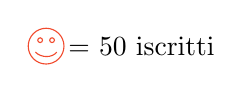
\begin{tikzpicture}
\begin{scope}[RedOrange]
\draw(0,-.5ex) circle (1.5ex);
\foreach \x in {-.5ex,.5ex}
  \draw[fill=white] (\x,0) circle (.2ex);
   \draw (-.9ex,-1ex)..controls (-0.4ex,-1.5ex)and(0.5ex,-1.5ex)..(.9ex,-1ex);
\end{scope}
\node () at (8ex,-.5ex) { $=$ 50 iscritti};
\end{tikzpicture}

\end{center}
Il numero degli iscritti di ogni anno scolastico sarà rappresentato da 
tante unità grafiche quanti sono i gruppi di~50 iscritti.
Per avere il grafico relativo all'anno~2003-2004 si devono usare tre 
faccine, in quanto~$150: 50 = 3$.
\begin{center}
 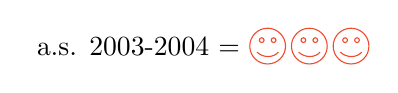
\begin{tikzpicture}
\begin{scope}[RedOrange]
\foreach \xi in {0,3.5ex,7ex}{
\draw(\xi,-.5ex) circle (1.5ex);
   \draw (\xi-.9ex,-1ex)..controls (\xi-0.4ex,-1.5ex)and(\xi+0.5ex,-1.5ex)..(\xi+.9ex,-1ex);}
\foreach \xii in {-.5ex,.5ex,3ex,4ex,6.5ex,7.5ex}
  \draw[fill=white] (\xii,0) circle (.2ex);
\end{scope}
\node[left] at (-1.5ex,-.5ex) { a.s. 2003-2004 $=$};
\end{tikzpicture}
\end{center}
Se la divisione del numero degli iscritti per~50 dà resto, esso si dovrà 
rappresentare disegnando solo una parte
dell'unità grafica, corrispondente alla frazione tra resto e~50. Ad esempio 
nell'~a.s.~2006-2007 ci sono stati~325 iscritti; $325:50 = 6$
col resto di~25, quindi~325 sarà uguale a~6 unità grafiche 
e~$\frac{25}{50}=\frac{1}{2}$ unità grafica, cioè mezza faccina.
\begin{center}
 % (c) 2012 Dimitrios Vrettos - d.vrettos@gmail.com

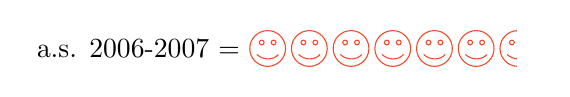
\begin{tikzpicture}
\begin{scope}[RedOrange]
\foreach \xi in {0,3.5ex,7ex,10.5ex,14ex,17.5ex,21ex}{
\draw(\xi,-.5ex) circle (1.5ex);
   \draw (\xi-.9ex,-1ex)..controls (\xi-0.4ex,-1.5ex)and(\xi+0.5ex,-1.5ex)..(\xi+.9ex,-1ex);}
\foreach \xii in {-.5ex,.5ex,3ex,4ex,6.5ex,7.5ex,10ex,11ex,13.5ex,14.5ex,17ex,18ex,20.5ex,21.5ex}
  \draw[fill=white] (\xii,0) circle (.2ex);
\end{scope}
\filldraw[white] (21ex,-2.2ex) rectangle (23ex,1.2ex);
\node[left] at (-1.5ex,-.5ex) { a.s. 2006-2007 $=$};
\end{tikzpicture}
\end{center}

Il grafico completo sarà:
\begin{center}
 % (c) 2012 Dimitrios Vrettos - d.vrettos@gmail.com

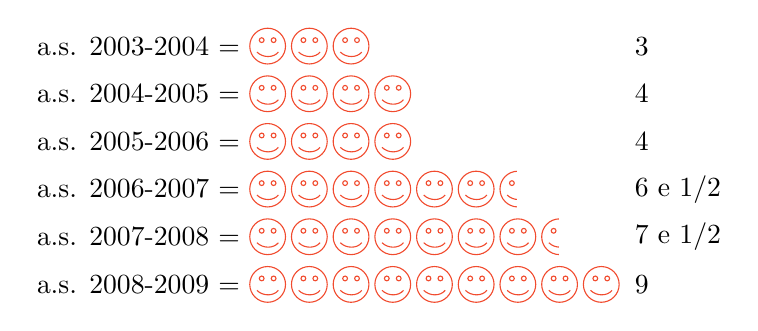
\begin{tikzpicture}[RedOrange]
  \foreach \xi in {0,3.5ex,7ex}{
    \draw(\xi,-.5ex) circle (1.5ex);
    \draw (\xi-.9ex,-1ex)..controls (\xi-0.4ex,-1.5ex)and(\xi+0.5ex,-1.5ex)..(\xi+.9ex,-1ex);
  }
  \foreach \xii in {-.5ex,.5ex,3ex,4ex,6.5ex,7.5ex}
    \draw[fill=white] (\xii,0) circle (.2ex);
  
  \node[left,black] at (-1.5ex,-.5ex) { a.s. 2003-2004 $=$};
  \node[right,black] at(30ex,-.5ex){3};

  \begin{scope}[yshift=-4ex]
    \foreach \xi in {0,3.5ex,7ex,10.5ex}{
      \draw(\xi,-.5ex) circle (1.5ex);
      \draw (\xi-.9ex,-1ex)..controls (\xi-0.4ex,-1.5ex)and(\xi+0.5ex,-1.5ex)..(\xi+.9ex,-1ex);
    }
    \foreach \xii in {-.5ex,.5ex,3ex,4ex,6.5ex,7.5ex,10ex,11ex}
      \draw[fill=white] (\xii,0) circle (.2ex);
    \node[left,black] at (-1.5ex,-.5ex) { a.s. 2004-2005 $=$};
    \node[right,black] at(30ex,-.5ex){4};
  \end{scope}

  \begin{scope}[yshift=-8ex]
    \foreach \xi in {0,3.5ex,7ex,10.5ex}{
      \draw(\xi,-.5ex) circle (1.5ex);
      \draw (\xi-.9ex,-1ex)..controls (\xi-0.4ex,-1.5ex)and(\xi+0.5ex,-1.5ex)..(\xi+.9ex,-1ex);}
    \foreach \xii in {-.5ex,.5ex,3ex,4ex,6.5ex,7.5ex,10ex,11ex}
      \draw[fill=white] (\xii,0) circle (.2ex);
    \node[left,black] at (-1.5ex,-.5ex) { a.s. 2005-2006 $=$};
    \node[right,black] at(30ex,-.5ex){4};
  \end{scope}

  \begin{scope}[yshift=-12ex]
    \foreach \xi in {0,3.5ex,7ex,10.5ex,14ex,17.5ex,21ex}{
      \draw(\xi,-.5ex) circle (1.5ex);
      \draw (\xi-.9ex,-1ex)..controls (\xi-0.4ex,-1.5ex)and(\xi+0.5ex,-1.5ex)..(\xi+.9ex,-1ex);}
    \foreach \xii in {-.5ex,.5ex,3ex,4ex,6.5ex,7.5ex,10ex,11ex,13.5ex,14.5ex,17ex,18ex,20.5ex,21.5ex}
      \draw[fill=white] (\xii,0) circle (.2ex);
    \node[left, black] at (-1.5ex,-.5ex) { a.s. 2006-2007 $=$};\filldraw[white] (21ex,-2.2ex) rectangle (23ex,1.2ex);
    \node[right,black] at(30ex,-.5ex){6 e  1/2};
  \end{scope}

  \begin{scope}[yshift=-16ex]
    \foreach \xi in {0,3.5ex,7ex,10.5ex,14ex,17.5ex,21ex,24.5ex}{
      \draw(\xi,-.5ex) circle (1.5ex);
      \draw (\xi-.9ex,-1ex)..controls (\xi-0.4ex,-1.5ex)and(\xi+0.5ex,-1.5ex)..(\xi+.9ex,-1ex);}
    \foreach \xii in {-.5ex,.5ex,3ex,4ex,6.5ex,7.5ex,10ex,11ex,13.5ex,14.5ex,17ex,18ex,20.5ex,21.5ex,24ex,25ex}
      \draw[fill=white] (\xii,0) circle (.2ex);
    \node[left, black] at (-1.5ex,-.5ex) { a.s. 2007-2008 $=$};\filldraw[white] (24.5ex,-2.2ex) rectangle (26.5ex,1.2ex);
    \node[right,black] at(30ex,-.5ex){7 e  1/2};
  \end{scope}

  \begin{scope}[yshift=-20ex]
    \foreach \xi in {0,3.5ex,7ex,10.5ex,14ex,17.5ex,21ex,24.5ex,28ex}{
      \draw(\xi,-.5ex) circle (1.5ex);
      \draw (\xi-.9ex,-1ex)..controls (\xi-0.4ex,-1.5ex)and(\xi+0.5ex,-1.5ex)..(\xi+.9ex,-1ex);}
    \foreach \xii in {-.5ex,.5ex,3ex,4ex,6.5ex,7.5ex,10ex,11ex,13.5ex,14.5ex,17ex,18ex,20.5ex,21.5ex,24ex,25ex,27.5ex,28.5ex}
      \draw[fill=white] (\xii,0) circle (.2ex);
    \node[left, black] at (-1.5ex,-.5ex) { a.s. 2008-2009 $=$};
    \node[right,black] at(30ex,-.5ex){9};
    \end{scope}
\end{tikzpicture}
\end{center}
 \end{esempio}
% \end{exrig}

\subsubsection{Diagramma a barre o a colonne}
Questo tipo di rappresentazione, detta anche diagramma a nastri o a 
bastoni, viene usata quando si vuole fornire un'idea delle frequenze
delle diverse modalità di un fenomeno, in genere si usa per caratteri 
qualitativi o quantitativi discreti.
Per poter valutare il significato statistico della lunghezza dei nastri o 
delle colonne è necessario scegliere opportunamente una scala di 
riferimento:
la larghezza del nastro è arbitraria ma uguale per tutti i nastri, la 
lunghezza è proporzionale alla caratteristica che si deve rappresentare.
I nastri e le colonne possono inoltre essere suddivisi in parti di colori 
diversi per indicare le singole componenti o i singoli fenomeni
che si vogliono analizzare.

La differenza fra la rappresentazione a barre e quella a colonne, detta 
anche istogramma, consiste soltanto
nell'orientamento del grafico: nel diagramma a nastri si indicano le 
modalità del carattere sull'asse verticale e le frequenze sull'asse 
orizzontale,
mentre in quello a colonne le modalità del carattere sono riportate 
sull'asse
orizzontale e le frequenze su quello verticale.

Di seguito vengono riportate le due tipologie di grafico accompagnate dalla 
tabella di riferimento:

\begin{center}
 \begin{tabularx}{.95\textwidth}{X*{7}{c}Xc}
\toprule
Materia& Italiano &Storia & Geografia & Matem. & Scienze & Ed. Fisica & 
Totale\\
Maschi & 5 & 4& 4 & 2& 6 & 5& 26\\
Femmine & 3 & 7 & 2 & 3  & 4 & 5 & 24\\
\bottomrule
\end{tabularx}
\end{center}
\begin{center}
\begin{figure}[!h]
\begin{minipage}{.5\textwidth}
\begin{inaccessibleblock}[Figura: TODO]
% (c) 2012 Dimitrios Vrettos - d.vrettos@gmail.com

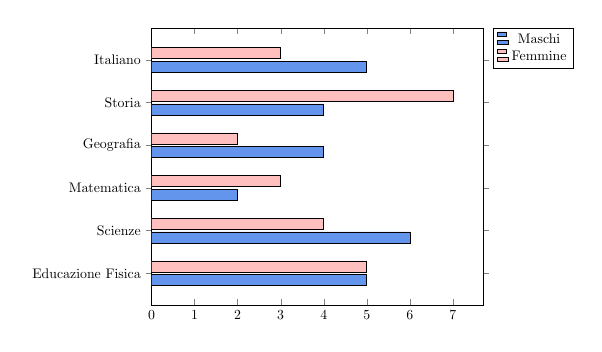
\begin{tikzpicture}[scale=.5]
\begin{axis}[
legend entries={Maschi, Femmine},
legend pos=outer north east,
xbar,
enlarge y limits=0.15,
symbolic y coords={Educazione Fisica,Scienze,Matematica, Geografia,Storia,Italiano },
ytick=data,
bar width=8pt, 
xmin=0, 
width=100mm]

\addplot[fill=CornflowerBlue, draw=black] coordinates {
(5,Educazione Fisica)
(6,Scienze)
(2,Matematica)
(4,Geografia)
(4,Storia)
(5,Italiano)
};

\addplot[fill=pink, draw=black] coordinates{
(5,Educazione Fisica)
(4,Scienze)
(3,Matematica)
(2,Geografia)
(7,Storia)
(3,Italiano)
};
\end{axis}
\end{tikzpicture}
\caption{Diagramma a barre}
\end{inaccessibleblock}
\end{minipage} 
\begin{minipage}{.5\textwidth}
\begin{inaccessibleblock}[Figura: TODO]
 % (c) 2012 Dimitrios Vrettos - d.vrettos@gmail.com

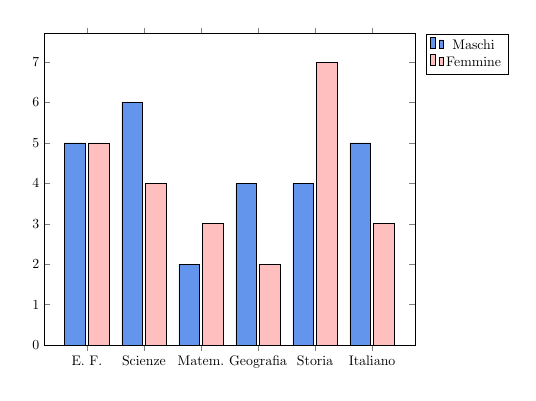
\begin{tikzpicture}[scale=.5]
\begin{axis}[
legend entries={Maschi, Femmine},
legend pos=outer north east,
ybar,
enlarge x limits=0.15,
symbolic x coords={E. F.,Scienze,Matem., Geografia,Storia,Italiano },
xtick=data,
bar width=15pt, 
ymin=0, 
width=110mm]

\addplot[fill=CornflowerBlue, draw=black] coordinates {
(E. F.,5)
(Scienze,6)
(Matem.,2)
(Geografia,4)
(Storia,4)
(Italiano,5)
};
 
 \addplot[fill=pink, draw=black] coordinates{
 (E. F.,5)
 (Scienze,4)
 (Matem.,3)
 (Geografia,2)
 (Storia,7)
 (Italiano,3)
 };
\end{axis}
\end{tikzpicture}
\caption{Diagramma a colonne}
\end{inaccessibleblock}
\end{minipage}
\end{figure} 

\end{center}

\subsubsection{Areogramma}
Questo tipo di rappresentazione viene utilizzato quando si vogliono 
evidenziare le parti che compongono un fenomeno, per esempio per indicare
come si dividono gli alunni di una classe in maschi e femmine, o per 
rappresentare in che modo
le varie voci di spesa incidono sul bilancio familiare.
Il grafico si ottiene dividendo un cerchio in settori circolari con aree 
direttamente proporzionali alle frequenze che rappresentano.
Per disegnare l'areogramma, si disegna una circonferenza di diametro 
arbitrario e si fa corrispondere l'angolo al centro di~$360\grado$,
con il~$100\%$ di frequenza percentuale; per ottenere gli angoli 
corrispondenti a frequenze percentuali minori, si risolve la 
proporzione~$360\grado:X\grado=100:X$.
Si suddivide così la circonferenza negli angoli ottenuti e si colorano o 
retinano diversamente i settori circolari ottenuti.

% \begin{exrig}
 \begin{esempio}
Consideriamo la seguente tabella statistica che indica gli studenti, divisi 
per classe, frequentata di un dato istituto scolastico, in un dato anno.

\begin{center}
\begin{tabular}{lcccccc}
\toprule
Classe & 1$\grado$ &2$\grado$ &3$\grado$ & 4$\grado$ &5$\grado$ &Totale\\
Studenti & 320 & 230 & 212 & 152 & 96 & 1010 \\
\bottomrule
\end{tabular}
\end{center}

Nella tabella sono indicate le frequenze assolute; calcoliamo ora le 
frequenze percentuali degli studenti.
Per la~1$\grado$ classe si ha:~$\frac{320}{1010}=0,32$ arrotondato alla 
seconda cifra decimale, che equivale al~$32\%$ e così via per le classi 
successive.

\begin{center}
\begin{tabular}{lcccccc}
\toprule
Classe & 1$\grado$ & 2$\grado$ & 3$\grado$ & 4$\grado$ & 5$\grado$ & Totale 
\\
 Frequenze percentuali& 32,00\% & 23,00\% & 21,00\% & 15,00\% & 9,00\% & 
100\% \\
\bottomrule
\end{tabular}
\end{center}

Rappresentiamo graficamente mediante areogramma i dati contenuti nella 
tabella precedente.
\begin{center}
 \begin{tikzpicture}[scale=.8, x=10mm,y=10mm, x radius=10mm, y radius=10mm]
  \draw (0,0) circle (3);
  \draw[pattern=north east lines,pattern color=orange] (0,0) -- (0:3) arc (0:115.2:3);
  \draw[pattern=horizontal lines,pattern color=brown] (0,0)-- (115.2:3) arc (115.2:198:3);
  \draw[pattern=dots,pattern color=green] (0,0)-- (198:3) arc (198:273.6:3);
  \draw[pattern=north west lines,pattern color=red] (0,0)-- (273.6:3) arc (273.6:327.6:3);
  \draw[pattern=vertical lines,pattern color=blue] (0,0)-- (327.6:3) arc (327.6:360:3);

  \begin{scope}[every node/.style={rounded corners, draw=black, fill=white}]
    \draw(57.6:2) node {$115,2\grado $};
    \draw(156.6:2) node {$82,8\grado $};
    \draw(235.8:2) node {$75,6\grado $};
    \draw(300.6:2) node {$54\grado $};
    \draw(343.8:2) node {$32,4\grado $};
  \end{scope}

  \begin{scope}[thick, <->]
    \draw (0:1) arc (0:115.2:1);
    \draw (115.2:.8) arc (115.2:198:.8);
    \draw (198:1.2) arc (198:273.6:1.2);
    \draw (273.6:.8) arc (273.6:327.6:.8);
    \draw (327.6:1.1) arc (327.6:360:1.1);
  \end{scope}

  \draw(57.6:4) node {1\textsuperscript{A} Classe: $32\%$};
  \draw[left](156.6:3) node {2\textsuperscript{A} Classe: $23\%$};
  \draw(235.8:4) node {3\textsuperscript{A} Classe: $21\%$};
  \draw[below right](300.6:3) node {4\textsuperscript{A} Classe: $15\%$};
  \draw[right](343.8:3) node {5\textsuperscript{A} Classe: $9\%$};
\end{tikzpicture}
\end{center}
Per ottenere l'angolo relativo alla frequenza percentuale 
della~1\textsuperscript{A} 
classe si fa:~$360\grado \cdot \frac{32}{100}=115,2\grado$ e per 
la~2\textsuperscript{A} classe:~$360\grado \cdot \frac{23}{100}=82,2\grado$ e 
cosi via per le altre classi.

Dal grafico si può notare immediatamente che la classe frequentata di più è 
la prima.

 \end{esempio}
% \end{exrig}

\subsubsection{Istogramma}
Si utilizza la rappresentazione grafica attraverso istogramma quando il 
carattere analizzato è di tipo quantitativo ed i dati sono raggruppati in 
classi.

Prima di tutto si distribuiscono i dati in classi o gruppi e si determina 
il numero di individui appartenenti a ciascuna classe, questo numero è
detto \emph{frequenza della classe}.
Riportando tali dati in una tabella si ottiene la distribuzione delle 
frequenze. Poiché le classi potrebbero avere ampiezze diverse si calcola
la \emph{densità di frequenza}, definita come rapporto fra la frequenza 
della classe e la relativa ampiezza.

Per disegnare un istogramma si tracciano due assi; sull'asse verticale, 
orientato verso l'alto, si fissa un segmento unitario e si riportano
le frequenze. L'asse orizzontale, orientato verso destra, è invece 
suddiviso in tanti segmenti la cui ampiezza è pari a quella delle singole 
classi.
Il grafico consiste in un insieme di rettangoli aventi per base ogni classe 
e altezza la densità di frequenza corrispondente.
In tal modo l'area di ogni rettangolo rappresenta la frequenza 
corrispondente a ciascuna classe.

% \begin{exrig}
 \begin{esempio}

Costruiamo un istogramma a partire dalla distribuzione di frequenza 
riportata nella seguente tabella:
\begin{center}
\begin{tabular}{lcc}
\toprule
Diametro crateri lunari ($\unit{km}$) & Numero di crateri\\
\midrule
$0-50$ & 1088 \\
$50-100$ & 745 \\
$100-150$ & 20 \\
\bottomrule
\end{tabular}
\end{center}

Innanzitutto dobbiamo determinare per ogni classe la densità di frequenza 
che si ottiene dividendo la frequenza assoluta per l'ampiezza della classe:

\begin{center}
\begin{minipage}{.6\textwidth}
\begin{tabular}{cc}
\toprule
Diametro crateri lunari ($\unit{km}$) & Densità\\
\midrule
$0-50$ & $1088/50=21,76$ \\
$50-100$ & $745/50=14,9$ \\
$100-150$ & $20/50=0,4$ \\
\bottomrule
\end{tabular}
\end{minipage} 
\begin{minipage}{.38\textwidth}
\begin{inaccessibleblock}[Figura: TODO]
% (c) 2012 Dimitrios Vrettos - d.vrettos@gmail.com

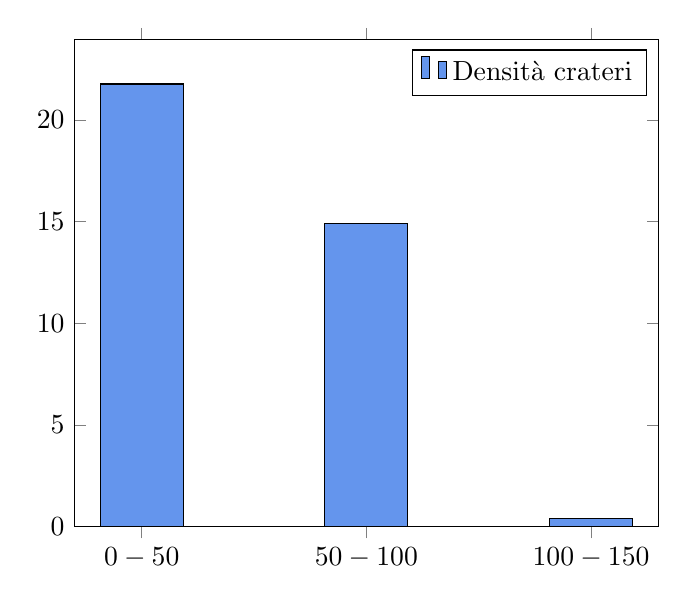
\begin{tikzpicture}
\begin{axis}[
legend entries={Densità crateri},
ybar,
enlarge x limits=0.15,
symbolic x coords={$0-50$,$50-100$,$100-150$},
xtick=data,
bar width=30pt, 
ymin=0, 
width=90mm]

\addplot[fill=CornflowerBlue, draw=black] coordinates {
($0-50$,21.76)
($50-100$,14.9)
($100-150$,.4)
 };
 
\end{axis}
\end{tikzpicture}
\end{inaccessibleblock}
\end{minipage}
\end{center}

\end{esempio}

% \end{exrig}

% \ovalbox{\risolvii \ref{ese:A.10}, \ref{ese:A.11}, \ref{ese:A.12}, 
% \ref{ese:A.13}, \ref{ese:A.14}, \ref{ese:A.15}, \ref{ese:A.16}, 
% \ref{ese:A.17}, \ref{ese:A.18}, \ref{ese:A.19}, \ref{ese:A.20}}

\section{Indici di posizione}
\label{sec:c_stat_posizione}

Gli indici di posizione vengono utilizzati per sintetizzare i dati di una 
distribuzione di frequenza per mezzo di un solo numero.
A seconda del tipo di carattere oggetto dell'indagine statistica possono 
essere utilizzati valori medi diversi.

\subsection{Moda}

\begin{definizione}
La \emph{moda} è la modalità del carattere indagato che si presenta più 
frequentemente.
\end{definizione}

In una successione di~$n$ modalità~$x_1, x_2, \ldots, x_n$
con le relative frequenze~$f_1, f_2, \ldots, f_n$, la moda è la modalità 
che ha la frequenza maggiore.
Questo valore può essere calcolato per qualunque tipo di carattere, sia 
qualitativo che quantitativo.
Se il carattere è quantitativo continuo con dati raggruppati in classi non 
è possibile determinare con esattezza la moda, ci si limita
ad individuare la classe modale definita come la classe cui è associata la 
massima densità di frequenza.

% \begin{exrig}

\begin{esempio}
La tabella raccoglie i dati relativi alla domanda ``quante ore la settimana 
pratichi sport?'', posta ad un
campione di~50 ragazzi dai~18 ai~25 anni. Si può osservare che~12 e~18 ore 
presentano la frequenza massima~14, quindi si hanno due
mode~12 ore e~18 ore. La distribuzione è bimodale.


\begin{center}
\begin{tabular}{lcccccccc}
\toprule
Numero di ore & 0 &4 &8 &12 &16 &18 &22 &Totale\\
 Numero di ragazzi& 4 & 1 & 3 & 14 & 8 & 14 & 6 & 50 \\
\bottomrule
\end{tabular}
\end{center}
 \end{esempio}

 \begin{esempio}
La tabella seguente è relativa alla distribuzione delle altezze di un 
gruppo di studenti.

\begin{center}
\begin{tabular}{lcccccc}
\toprule
Altezza &160-165 &165-170 &170-175 &175-185 &185-200 &Totale \\
Numero di studenti & 5 & 8 & 15 & 10 & 2 & 40 \\
\bottomrule
\end{tabular}
\end{center}
Poiché le classi hanno ampiezza diversa è necessario calcolare la densità 
di frequenza.

\begin{center}
\begin{tabular}{lccccc}
\toprule
Altezza &160-165 &165-170 &170-175 &175-185 &185-200 \\
Densità di frequenza & 1 & 1,6 & 3 & 1 & 0,13 \\
\bottomrule
\end{tabular}
\end{center}
La massima densità di frequenza si ha in corrispondenza della 
classe~170-175, essa rappresenta quindi la classe modale.
 \end{esempio}
% \end{exrig}

\subsection{Media aritmetica}

\begin{definizione}
La \emph{media aritmetica} semplice o media aritmetica è il valore ottenuto 
sommando tutti i dati e
dividendo tale somma per il numero dei dati.
\end{definizione}

Se abbiamo~$n$ dati~$x_1, x_2, \ldots, x_n$ la media aritmetica 
semplice~$M$ è:

\begin{equation*}
M=\frac{x_1+x_2+ \dots +x_n}{n}=\frac{1}{n}\sum_{i=1}^n x_i.
\end{equation*}

% \begin{exrig}
 \begin{esempio}

Riprendiamo in esame la tabella relativa agli studenti, divisi per classe 
frequentata di un dato istituto scolastico, in un dato anno. Calcoliamo la 
media aritmetica semplice.
\begin{center}
 \begin{tabular}{lcccccc}
 \toprule
 Classe & 1$\grado$ & 2$\grado$ & 3$\grado$ & 4$\grado$ & 5$\grado$ & 
Totale\\
 Studenti & 320 & 230 & 212 & 152 & 96 & 1010\\
 \bottomrule
\end{tabular}
\end{center}
Per calcolare la media aritmetica semplice degli studenti, sommiamo tutti 
gli studenti delle cinque classi e dividiamo tale somma per il numero delle 
classi:
\begin{equation*}
M=\frac{320+230+212+152+96}{5}= \frac{1010}{5}= 202.
\end{equation*}
Possiamo dire che \emph{in media} si hanno~202 studenti per ogni classe.

\begin{definizione}
Si definisce \emph{scarto dalla media} (aritmetica) la differenza tra i 
valori osservati e la media.
\end{definizione}

Se~$x_1, x_2, \ldots, x_n$ sono i valori osservati, $M$ la media 
aritmetica, gli scarti sono~$s_1=x_1-M$, $s_2=x_2-M$, \ldots, $s_n=x_n-M$.
\end{esempio}

\begin{esempio}
Calcoliamo gli scarti dalla media per la distribuzione ``studenti per 
tipologia di classe frequentata'', la cui media è~$1010/5 = 202$.
\begin{center}
\begin{tabular}{l*{6}{c}}
\toprule
Classe & 1$\grado$ & 2$\grado$ & 3$\grado$ & 4$\grado$ & 5$\grado$ & 
Totale\\
Studenti & 320& 230& 212& 152& 96& 1010 \\
Scarto & 118 & 28 & 10 & $-50$ & 106 & 0\\
\bottomrule
\end{tabular}
\end{center}
Si può osservare che vi solo valori superiori alla media e altri inferiori, 
tanto che lo scarto è rappresentato in
alcuni casi da un numero positivo, in altri da un numero negativo. Si può 
verificare che la somma degli scarti è nulla,
cioè gli scarti positivi compensano sempre quelli negativi.
 \end{esempio}
% \end{exrig}

\begin{definizione}
La \emph{media aritmetica ponderata} è il valore ottenuto moltiplicando 
ciascun dato con la propria
frequenza, sommando tutti i prodotti fra loro e dividendo tale somma per il 
numero totale dei dati.
\end{definizione}

Essa si usa nel caso in cui i dati sono molti ed è già stata fatta la 
tabella delle frequenze. In questo caso,
avendo~$n$ dati~$x_1, x_2, \ldots, x_n$ con le relative frequenze~$f_1, 
f_2, \ldots, f_n$, la media aritmetica ponderata~$M$ è:
\begin{equation*}
M=\frac{x_1\cdot f_1+x_2\cdot f_2+ \dots +x_n\cdot f_n}{f_1+f_2+ \dots 
+f_n}=\frac{1}{n}\sum_{i=1}^n x_i\cdot f_i.
\end{equation*}
% \begin{exrig}
 \begin{esempio}

Riprendiamo la tabella dell'esempio precedente relativa alla domanda 
``quante ore al giorno passi al computer?'',
posta ad un campione di~52 ragazzi dai~16 ai~24 anni. Calcoliamo la media 
aritmetica ponderata.

\begin{center}
 \begin{tabular}{lcccccccc}
 \toprule
 Numero di ore & 0 & 1 & 2 & 3 & 4 & 5 & 6 & Totale\\
 Numero di ragazzi & 4 & 6 & 12 & 16 & 8 & 4 & 2 & 52\\
 \bottomrule
\end{tabular}
\end{center}

Calcoliamo la media aritmetica ponderata:
\begin{equation*}
M=\frac{0\cdot 4+1\cdot 6+2\cdot 12+3\cdot 16+4\cdot 8+5\cdot 4+6\cdot 
2}{4+6+12+16+8+4+2}=\frac{142}{52}=2,73.
\end{equation*}

Possiamo dire che ``in media'' ciascun ragazzo passa circa~3 ore al giorno 
al computer.
\end{esempio}
% \end{exrig}

\subsection{Mediana}
\begin{definizione}
La \emph{mediana} di una successione di dati disposti in ordine crescente è 
il dato che occupa la
posizione centrale se il numero dei dati è dispari; se il numero dei dati è 
pari è la media aritmetica dei dati della coppia centrale.
\end{definizione}

Poiché per calcolare la mediana i dati devono essere ordinati, è bene 
sottolineare che tale valore medio non può essere calcolato se il carattere
in esame è di tipo qualitativo non ordinabile.

% \begin{exrig}
\begin{esempio}
Supponiamo di avere~7 dati disposti in ordine crescente: 5, 8, 10, 14, 18, 
20, 25.
Allora la mediana è il valore centrale, quello che occupa la quarta 
posizione, il~14.
\end{esempio}

\begin{esempio}
Supponiamo di avere~8 dati disposti in ordine crescente: 1, 5, 8, 10, 14, 
18, 20, 25.
La mediana è la media aritmetica dei dati che occupano la~4$\grado$ e 
la~5$\grado$ posizione, cioè~$\frac{10+14}{2}=12$.
\end{esempio}

\begin{esempio}
Supponiamo di avere la distribuzione di frequenza riportata nella tabella.
Il numero di osservazioni è pari, quindi la mediana è il valore della 
variabile che corrisponde alla media dei due
valori centrali, rispettivamente quelli che nella serie ordinata occupano 
il~13$\grado$ e il~14$\grado$ posto.

È necessario in questo caso determinare le \emph{frequenze cumulate}, esse 
si ottengono sommando le frequenze che hanno un valore della
variabile minore o uguale alla modalità corrispondente.
La frequenza cumulata relativa al voto~3 rimane~2, quella relativa al 
voto~4 si ottiene sommando
la frequenza del~3 e la frequenza del~4, cioè~$2+2=4$, la frequenza 
cumulata relativa al voto~5 si ottiene dalla somma
della frequenza del~3, del~4 e del~5 e così via. Il~14$\grado$ posto 
corrisponde al voto~6, mentre il~15$\grado$ posto è il voto~7.
La mediana è~6,5.
\begin{center}
\begin{tabular}{ccl}
\toprule
Voto & Frequenza & Frequenza cumulata\\
\midrule
3 & 2 & 2 \\
4 & 4 & 4+2=6 \\
5 & 3 & 3+4+2=9 \\
6 & 5 & 5+3+4+2=14 \\
7 & 7 & 7+5+3+4+2=21 \\
8 & 2 & 2+7+5+3+4+2=23 \\
9 & 2 & 2+2+7+5+3+4+2=25 \\
10 & 1 & 1+2+2+7+5+3+4+2=26 \\
\midrule
Totale & 26 & \\
\bottomrule
\end{tabular}
\end{center}
\end{esempio}
% \end{exrig}

% \ovalbox{\risolvii \ref{ese:A.21}, \ref{ese:A.22}, \ref{ese:A.23}, 
% \ref{ese:A.24}, \ref{ese:A.25}, \ref{ese:A.26}, \ref{ese:A.27}, 
% \ref{ese:A.28}, \ref{ese:A.29}, \ref{ese:A.30}, \ref{ese:A.31}}

% \vspazio\ovalbox{\ref{ese:A.32}}

\section{Indici di variabilità}
\label{sec:c_stat_variabilita}

Gli \emph{indici di variabilità} vengono calcolati per analizzare in che 
modo i termini di una distribuzione si concentrano intorno ad un valore 
medio.

\begin{definizione}
Il \emph{campo di variazione} è la differenza fra il valore massimo ed il 
valore minimo assunti dalla
variabile: $\cvar = x_{max} - x_{min}$.
\end{definizione}

Tale indice dà un'informazione molto grossolana perché tiene conto solo del 
primo e dell'ultimo termine della
distribuzione e non tiene conto di tutti i valori intermedi. Si 
considerino, ad esempio, le seguenti distribuzioni di stature:
\begin{center}
 \begin{tabular}{lccccccc}
 \toprule
 Gruppo A (statura in~$\unit{cm}$) & 150 & 155 & 155 & 160 & 165 & 180 & 
175 \\
 Gruppo B (statura in~$\unit{cm}$) & 150 & 160 & 175 & 170 & 170 & 170 & 
180 \\
 \bottomrule
\end{tabular}
\end{center}

Entrambe le distribuzioni hanno lo stesso valore massimo e lo stesso valore 
minimo e quindi lo stesso campo di
variazione, ma mentre nella prima i valori sono concentrati verso il valore 
minimo nella seconda si concentrano intorno al valore massimo.

L'indice non dà quindi alcuna indicazione su quest'ultima informazione. Né 
può essere utilizzato come indice di
variabilità la media degli scarti fra le singole osservazioni e la loro 
media aritmetica perché tale valore è sempre uguale a zero.

\subsection{Scarto medio assoluto}

\begin{definizione}
Si definisce \emph{scarto medio assoluto} la media aritmetica dei valori 
assoluti degli scarti; esso indica quanto i valori rilevati si disperdono
intorno al valore medio della distribuzione:
\[s=\frac{\valass{s_1}+\valass{s_2}+ \cdots +\valass{s_n}}{n}=\frac 
{1}{n}\sum_{i=1}^n \valass{x_i - M}.\]
\end{definizione}

Facendo riferimento alla distribuzione
\begin{center}
\begin{tabular}{lcccccc}
\toprule
 Classe & 1$\grado$ & 2$\grado$ & 3$\grado$ & 4$\grado$ & 5$\grado$ & 
Totale\\
 Studenti & 320 & 230 & 212 & 152 & 96 & 1010 \\
\bottomrule
\end{tabular}
\end{center}
si ha che lo scarto medio assoluto è~62,4. Si può allora affermare che in 
ogni tipologia di classe si hanno in media~$202\pm~62,4$ iscritti.

\subsection{Varianza e scarto quadratico medio}

L'indice più utilizzato è la varianza.

\begin{definizione}
La \emph{varianza} è la media dei quadrati degli scarti fra le singole 
osservazioni e la loro media
aritmetica:
\[\var=\frac{ \left[ (x_1-M)^2+(x_2-M)^2+ \cdots +(x_n-M)^2 \right] 
}{n}=\frac{1}{n}\sum_{i=1}^n (x_i-M)^2.\]

Lo \emph{scarto quadratico medio} è la radice quadrata della 
varianza:~$\sigma=\sqrt{\var{}}$.
\end{definizione}

Se i dati si presentano sotto forma di distribuzione di frequenza la media 
deve essere ponderata con le singole
frequenze, cioè:
\begin{equation*}
\var{}=\frac{\left[(x_1-M)^2\cdot f_1+(x_2-M)^2\cdot f_2+ \cdots 
+(x_n-M)^2\cdot f_n \right]}{f_1+f_2+\ldots+f_n}=\frac 
{1}{n}\sum_{i=1}^n(x_i-M)^2\cdot f_i.
\end{equation*}

La varianza assume valore zero quando tutti i valori coincidono con la 
media ed è tanto più grande quanto più i singoli valori
si discostano dalla media. Poiché tale indice è influenzato sia dal valore 
della media che dall'unità di misura utilizzato spesso si utilizza
un indice detto \emph{coefficiente di variazione}.

\subsection{Coefficiente di variazione}

\begin{definizione}
Il \emph{coefficiente di variazione} è uguale al rapporto fra scarto 
quadratico medio (radice quadrata
della varianza) e media aritmetica:
\[\cfvar{} = \frac{\sqrt{\var{}}}{\media}\].
\end{definizione}
Tale indice risulta di particolare utilità per confrontare distribuzioni 
diverse.

% \begin{exrig}
 \begin{esempio}

È dato l'elenco delle stature, in~$\unit{cm}$, dei ragazzi di
una classe: 165, 182, 159, 173, 160, 175, 185, 190, 175, 180, 159, 185, 
176, 170, 175, 160, 175, 182, 159, 185.

\begin{enumeratea}
\item Ordina i dati in una tabella delle frequenze;
\item rappresenta i dati graficamente;
\item calcola la media, la mediana e la moda;
\item calcola la varianza e il coefficiente di variazione.
\end{enumeratea}

\subsubsection{Tabella delle frequenze}

\begin{center}
\begin{tabular}{lccc}
\toprule
Dati & Frequenze assolute & Frequenze relative & Frequenze percentuali\\
\midrule
159 & 3 & 0,15 & 15\% \\
160 & 2 & 0,1 & 10\% \\
165 & 1 & 0,05 & 5\% \\
170 & 1 & 0,05 & 5\% \\
173 & 1 & 0,05 & 5\% \\
175 & 4 & 0,2 & 20\% \\
176 & 1 & 0,05 & 5\% \\
180 & 1 & 0,05 & 5\% \\
182 & 2 & 0,1 & 10\% \\
185 & 3 & 0,15 & 15\% \\
190 & 1 & 0,05 & 5\% \\
\midrule
Totale & 20 & 1 & 100\% \\
\bottomrule
\end{tabular}
\end{center}
\begin{itemize*}
\item La somma delle frequenze assolute indica il numero totale degli 
studenti;
\item la somma delle frequenze relative deve avvicinarsi il più possibile 
a~1;
\item la somma delle frequenze percentuali deve avvicinarsi il più 
possibile a~100.
\end{itemize*}
\vspace{-24pt}
\subsubsection{Grafici}
\begin{center}
 % (c) 2012 Dimitrios Vrettos - d.vrettos@gmail.com


\begin{tikzpicture}[scale=.8, x=7mm,y=7mm, x radius=7mm, y radius=7mm]
  \draw (0,0) circle (3);
  \draw[fill=orange] (0,0) -- (0:3) arc (0:54:3);
  \draw[fill=brown] (0,0)-- (54:3) arc (54:90:3);
  \draw[fill=green] (0,0)-- (90:3) arc (90:108:3);
  \draw[fill=red] (0,0)-- (108.6:3) arc (108:126:3);
  \draw[fill=blue] (0,0)-- (126:3) arc (126:144:3);
  \draw[fill=olive] (0,0)-- (144:3) arc (144:216:3);
  \draw[fill=lightgray] (0,0)-- (216:3) arc (216:234:3);
  \draw[fill=violet] (0,0)-- (234:3) arc (234:252:3);
  \draw[fill=lime] (0,0)-- (252:3) arc (252:288:3);
  \draw[fill=purple] (0,0)-- (288:3) arc (288:342:3);
  \draw[fill=pink] (0,0)-- (342:3) arc (342:360:3);
\node  at (0,4) {Areogramma};
\begin{scope}[xshift=28mm,
every node/.style={ anchor=center}]
\matrix[matrix of nodes] at (0,0){
\node[fill=orange]{};&159\\
\node[fill=brown]{};&160\\
\node[fill=green]{};&165\\
\node[fill=red]{};&170\\
\node[fill=blue]{};&173\\
\node[fill=olive]{};&175\\
\node[fill=lightgray]{};&176\\
\node[fill=violet]{};&180\\
\node[fill=lime]{};&182\\
\node[fill=purple]{};&185\\
\node[fill=pink]{};&190\\
};
\end{scope}

\begin{scope}[xshift=42mm, yshift=-21mm]
\pgfplotsset{width=7cm}
\begin{axis}[ymin=0]
    \addplot[color=blue, mark=*]
      coordinates{
	(159,3)
(160,2)
(165,1)
(170,1)
(173,1)
(175,4)
(176,1)
(180,1)
(182,2)
(185,3)
(190,1)
      };
\end{axis}

\node  at (3.5,7) {Diagramma Cartesiano};
\end{scope}
\end{tikzpicture}


\end{center}

\vspace{-24pt}
\subsubsection{Calcolo della media, mediana e moda}

Calcoliamo la media aritmetica:
\begin{equation*}
\begin{split}
\media &= \frac{1}{20} \cdot 
(165+182+159+173+160+175+185+190+175+180+159+185\\
 &+176+170+175+160+175+182+159+185)=173,5.
\end{split}
\end{equation*}

Per determinare la mediana si devono ordinare in modo crescente i dati:
159, 159, 159, 160, 160, 165, 170, 173, 175, 175, 175, 175, 176, 180, 182, 
182, 185, 185, 185, 190.
Essendo i dati in numero pari si calcola la media dei due dati centrali:
$\mediana = {175+175}/{2}=175.$
Se i dati sono molti è possibile individuare qual è o quali sono i dati 
centrali utilizzando la tabella delle
frequenze opportunamente costruita, cioè con i dati scritti in ordine 
crescente.

La moda è la modalità del carattere altezza che è più ricorrente, cioè 
quello con la frequenza più alta:
$\moda = 175$.
\end{esempio}
% \end{exrig}

% \ovalbox{\risolvii \ref{ese:A.33}, \ref{ese:A.34}, \ref{ese:A.35}, 
% \ref{ese:A.36}, \ref{ese:A.37}, \ref{ese:A.38}}


\section{Tabelle a doppia entrata}
\label{sec:c_stat_doppia_entrata}

La statistica descrittiva bivariata si occupa dell'analisi di due variabili 
congiuntamente considerate; in particolare, risulta interessante sapere se, 
e in quale modo, le due variabili si influenzano o se, al contrario, si 
manifestano una indipendentemente dall'altra.\\ 
A questo proposito verranno presentati, in seguito, alcuni indici in grado 
di interpretare il tipo di legame esistente tra due variabili. Prima di 
procedere risulta importante acquisire il concetto di distribuzione di 
frequenza bivariata. 
Si tratta di raccogliere i dati in una tabella a doppia entrata in grado di 
mostrare congiuntamente le modalità dei due caratteri.\\
Per la realizzazione degli esempi numerici contenuti nel capitolo, verranno 
utilizzati i seguenti dati ottenuti da una popolazione di n=20 individui 
che hanno partecipato ad un corso di tennis; le variabili rilevate sono 
\textquotedblleft voto (in trentesimi) ottenuto al termine del 
corso\textquotedblright (variabile quantitativa discreta), 
\textquotedblleft altezza in cm\textquotedblright (variabile quantitativa 
continua), \textquotedblleft sesso\textquotedblright (variabile qualitativa 
nominale), \textquotedblleft gradimento dell'organizzazione e della qualità 
dei maestri\textquotedblright (variabile qualitativa ordinale) e 
\textquotedblleft titolo di studio\textquotedblright (variabile qualitativa 
ordinale).

\begin{center}
        Variabili rilevate su ogni unità statistica
\end{center}
\begin{tabular}{|p{1.5cm}|c|c|c|c|c|}
\hline
        &Z&     Y       &X      &W      &L\\
        \hline
Unità statistiche &     Voto&   Altezza &Sesso& Gradimento&     Titolo di 
studio\\
\hline
        1&      196&    178,23  &Maschio&       Basso&  Licenza media\\
        \hline
        2&      19&     170,03& Maschio &Medio& Diploma\\
        \hline
        3&      22      &173,74 &Femmina&       Basso&  Diploma\\
        \hline
        4       &18&    171,26& Maschio&        Alto&   Licenza media\\
        \hline
        5&      24&     157,12& Femmina&        Alto&   Licenza media\\
        \hline
        6&      20      &163,76&        Femmina &Alto&  Licenza media\\
        \hline
        7&      21&     185,41& Maschio &Basso  &Diploma\\
        \hline
        8       &19&    175,53& Femmina&        Basso   &Diploma\\
        \hline
        9&      20&     182,97& Femmina&        Medio&  Licenza media\\
        \hline
        10&     21      &165,84&        Maschio&        Basso   &Licenza 
media\\
        \hline
        11      &22     &158,57 &Maschio&       Alto    &Diploma\\
        \hline
        12      &25     &188,05&        Maschio&        Alto&   Laurea I 
livello\\
        \hline
        13      &24&    178,88& Femmina&        Medio&  Laurea I livello\\
        \hline
        14      &19&    169,35& Maschio&        Medio&  Diploma\\
        \hline
        15      &22&    179,29& Femmina&        Basso&  Licenza media\\
        \hline
        16&     24      &157,20 &Femmina&       Basso&  Laurea I livello\\
        \hline
        17&     20      &187,42&        Femmina&        Medio&  Diploma\\
        \hline
        18      &25&    156,00& Maschio &Basso  &Laurea I livello\\
        \hline
        19&     23&     166,74& Femmina&        Alto&   Diploma\\
        \hline
        20&     19      &189,99&        Femmina &Alto&  Diploma\\
        \hline

\end{tabular}

\vspace{12pt}
La statistica descrittiva univariata ha come obiettivo lo studio della 
distribuzione di ogni variabile, singolarmente considerata, all'interno 
della popolazione (analisi per colonna) mentre la statistica descrittiva 
bivariata si occupa dello studio della distribuzione di due variabili 
congiuntamente considerate.

Si ipotizzi, ad esempio, di costruire la tabella a doppia entrata per le 
variabili X \textquotedblleft sesso\textquotedblright e W \textquotedblleft 
gradimento\textquotedblright:

\begin{tabular}{|c|c|c|c|c|}
\hline
 & W & W & W & \\
\hline
 & Basso & Medio & Alto & Somma\\
X &  & & &\\
 & $w_1$ & $w_2$ &  $w_3$ & \\
 \hline
 Femmina & 4 & 3 & 4 & 11\\
   &  & & &\\
 $x_1$ & $(n_{11})$ & $(n_{12})$ &  $(n_{13})$ & $n_1$ \\
  \hline
   Maschio & 4 & 2 & 3 & 9\\
   &  & & &\\
   $x_2$ & $(n_{21})$ & $(n_{22})$ &  $(n_{23})$ & $n_2$ \\
   \hline
 &  &  &  & \\
 Somma  & 8 & 5& 7&20\\
    & $n_{1}$ & $n_{2}$ &  $n_{3}$ & N \\   
  
  \hline
\end{tabular}

\vspace{6pt}
La tabella a doppia entrata mostra sulle righe le modalità della 
variabile X (\textquotedblleft femmina\textquotedblright e 
\textquotedblleft maschio\textquotedblright) e sulle colonne le modalità di 
W (\textquotedblleft basso\textquotedblright, \textquotedblleft 
medio\textquotedblright e \textquotedblleft alto\textquotedblright); la 
tabella, inoltre, è composta dalle seguenti distribuzioni:  

\begin{description} [noitemsep]
        \item [distribuzione congiunta di X e di W]: 
le frequenze congiunte (assolute) $n_{ij}$, 
che si trovano al centro della tabella, 
stanno ad indicare quante unità statistiche hanno manifestato 
contemporaneamente la modalità $x_i$ e la modalità $w_j$ (ad esempio, ci 
sono 4 femmine che hanno espresso un giudizio basso, ci sono 3 maschi con 
un giudizio alto e così via). Si osservi che il numero delle celle 
contenenti le frequenze congiunte è dato dal prodotto del numero di righe 
$h$ per il numero di colonne $k$, per cui la scrittura corretta prevede 
l'utilizzo del doppio pedice $n_{ij}$ ($i=1,2,\dots,k; j=1,2,\dots,h$);
        \item [distribuzione marginale di X]: 
considerando solamente 
la prima e l'ultima colonna della tabella a doppia entrata, si ottiene la 
distribuzione di frequenza marginale della variabile X, eliminando così 
l'effetto della variabile W. Le frequenze (assolute) della variabile X sono 
dette \emph{frequenze marginali (assolute)} e si indicano con $n_i$. 
($i=1,2,\dots,k$);
        \item [distribuzione marginale di W]: 
considerando solamente 
la prima e l'ultima riga della tabella a doppia entrata, si ottiene la 
distribuzione di frequenza marginale della variabile W, eliminando così 
l'effetto della variabile X. Le frequenze (assolute) della variabile W sono 
dette \emph{frequenze marginali (assolute)} e si indicano con $n_j$ 
($j=1,2,\dots,h$);
\end{description}

Qui di seguito vengono elencate tutte le restanti tabelle a doppia entrata 
costruibili con le variabili a disposizione contenute nella prima tabella:

\noindent
\begin{tabular}{|c|c|c|c|c|c|c|c|c|c|}
        \hline
X/Z&&&&&&&&&\\ 
\hline
        &18&    19&     20&     21&     22&     23&     24&     25&     
somma\\ 
        \hline
Femmina&        0&      2&      3&      0&      2       &1      &3      
&0      &11\\
\hline
Maschio&        1&      3&      0       &2      &1&     0&      0&      
2&      9\\
\hline
somma & 1&      5&      3&      2&      3&      1&      3       &2      
&20\\
\hline
\end{tabular}

\noindent
\begin{tabular}{|c|c|c|c|c|c|c|c|}
        \hline
        X/Z&&&&&&&\\ 
        \hline
&       {\scriptsize (155-160]}&        {\scriptsize (160-165]} 
&{\scriptsize (165-170]}&       {\scriptsize (170-175]} &{\scriptsize 
(175-180]}&     {\scriptsize (180-190]}&        {\scriptsize somma}\\
\hline 
Femmina&        2&      1&      1&      1&      3&      3&      11\\
\hline
Maschio&        2&      0&      2&      2&      1&      2&      9\\
\hline
somma&  4&      1&      3&      3&      4&      5&      20\\
        \hline
\end{tabular}

\noindent
\begin{tabular}{|c|c|c|c|c|c|c|c|c|c|}
        \hline
        W/Z&&&&&&&&&\\ 
        \hline
&       18&     19&     20&     21&     22&     23&     24&     25&     
somma\\ 
\hline
Basso&  0       &2&     0&      2       &2      &0      &1&1    &8\\
\hline
Medio & 0&      2&      2       &0&     0&      0       &1      &0&     5\\
\hline
Alto&   1&      1&      1&      0&      1&      1&      1&      1&      7\\
\hline
somma & 1&      5&      3&      2&      3       &1      &3      &2      
&20\\
\hline
\end{tabular}

\noindent
\begin{tabular}{|c|c|c|c|c|c|c|c|}
        \hline
        W/Y&&&&&&&\\ 
        \hline
&{\scriptsize   (155-160]}&     {\scriptsize (160-165]}&        
{\scriptsize (165-170]}&        {\scriptsize (170-175]} &{\scriptsize 
(175-180]}&     {\scriptsize (180-190]}&        {\scriptsize Somma}\\ 
\hline
Basso&  2&      0&      1&      1&      3&      1&      8\\
\hline
Medio & 0&      0&      1&      1&      1&      2&      5\\
\hline
Alto&   2&      1&      1&      1&      0&      2&      7\\
\hline
somma&  4&      1&      3&      3&      4&      5&      20\\
\hline
\end{tabular}

\noindent
\begin{tabular}{|c|c|c|c|c|c|c|c|c|c|}
        \hline
        Y/Z&&&&&&&&&\\ 
        \hline
&       18&     19&     20&     21&     22&     23&     24&     25&     
somma\\ 
\hline
(155-160]&      0       &0&     0&      0       &1&     0&      2&      
1&      4\\
\hline
(160-165]&      0       &0&     1&      0&      0&      0&      0&      
0&      1\\
\hline
(165-170]&      0&      1&      0&      1&      0&      1&      0&      
0&      3\\
\hline
(170-175]&      1       &1&     0&      0&      1&      0&      0&      
0&      3\\
\hline
(175-180]&      0&      2&      0&      0&      1&0&    1&      0&      4\\
\hline
(180-190]&      0&      1&      2&      1&      0&      0&      0&      
1&      5\\
\hline
somma&  1&      5&      3&      2&      3&      1&      3&      2&      20\\

        \hline
\end{tabular}

\vspace{6pt}
Si noti come una tabella possa essere costruita accoppiando variabili di 
diversa natura: qualitativa (nominale o ordinale) e qualitativa (nominale o 
ordinale), qualitativa (nominale o ordinale) e quantitativa (discreta o 
continua in classi), quantitativa (discreta o continua in classi) e 
quantitativa (discreta o continua in classi). A partire da una data tabella 
a doppia entrata sarà possibile affrontare lo studio dei vari legami tra 
variabili.

\section{Indipendenza e connessione}
\label{sec:c_stat_indipendenza_connessione}

\subsection{L'indipendenza statistica}

L'indipendenza statistica è il concetto base della statistica bivariata.

Data una tabella a doppia entrata, due variabili X e Y si dicono 
\textbf{indipendenti} se le modalità di X non influenzano il verificarsi 
delle modalità di Y, e viceversa (per questo si dice che l'indipendenza 
statistica è una relazione bidirezionale: se X è indipendente da Y anche Y 
è indipendente da X). In caso contrario, ovvero in assenza di indipendenza 
statistica, si parla genericamente di connessione: le due variabili X e Y 
tendono ad influenzarsi reciprocamente e tra di loro esiste una qualche 
relazione generica. Per questo motivo, l'indipendenza statistica e la 
\emph{connessione} sono concetti che si escludono reciprocamente.

\subsection{Il Chi quadro}

L'indice per l'indipendenza statistica viene chiamato \emph{Chi quadro}.

La presenza di indipendenza statistica o di connessione tra due variabili X 
e Y si misura con l'indice Chi Quadro $\chi^2$, che si basa sul confronto 
tra le frequenze assolute osservate  $n_{ij}$ (contenute nella tabella) e 
le frequenze teoriche $n^*_{ij}$ che si osserverebbero in caso di 
\emph{indipendenza} tra X e Y (le frequenze teoriche vanno calcolate 
in una nuova tabella  tramite la relazione $n^*_{ij}=\frac{n_i\cdot 
n_j}{n}$ $(i=1,2,\dots,k; j=1,2,\dots,h)$. La formula per il calcolo 
dell'indice è data dalla seguente espressione: 
$$\chi^2=\frac{\sum_{i=1}^{k}\sum_{j=1}^{h}\left( n_{ij}-n^*_{ij}\right) 
^2}{n^*_{ij}}$$
se tutte le frequenze osservate $n_{ij}$ coincidono con le frequenze 
teoriche $n^*_{ij}$ siamo in presenza di indipendenza statistica ma, 
qualora anche solo una frequenza osservata fosse diversa dalla 
corrispondente frequenza teorica, potremmo escludere l'indipendenza ed 
affermare che esiste connessione tra X e Y.

\subsection{Il Chi quadro normalizzato}

 Per stabilire se la connessione tra X e Y è alta o bassa è possibile 
ricorrere alla normalizzazione dell'indice. Sapendo, infatti, che il minimo 
del Chi Quadro è 0 (in caso di indipendenza statistica) e il massimo è 
$n(min(h-1,k-1))$  (in caso di massima connessione), dove $k$ è il numero 
di righe della tabella, $h$ il numero di colonne, n la numerosità della 
popolazione e min la funzione minimo, l'indice normalizzato:
 $$\widetilde{\chi}^2=\frac{\chi^2}{n\cdot min(h-1,k-1)}$$
 assumerà valore 0 in caso di indipendenza statistica, valore 1 in caso di 
massima connessione, valori vicino a 0 nel caso di bassa connessione e 
valori vicino a 1 in presenza di alta connessione.

\begin{esempio}
Per una maggiore comprensione, presentiamo qui di seguito il calcolo 
dell'indice Chi quadro per la coppia di variabili (X,W).
Come primo passo si riporta la tabella delle frequenze osservate $n_{ij}$:

\begin{tabular}{|c|c|c|c|c|}
\hline
X/W &&&&\\
\hline
        &Basso& Medio&  Alto&   Somma\\ 
        \hline
Femmina&        4&      3&      4&      11\\
\hline
Maschio&        4&      2&      3&      9\\
\hline
somma&  8&      5       &7&     20\\
\hline

\end{tabular}

\vspace{6pt}
Successivamente si costruisce la tabella che contiene le frequenze teoriche 
$n^*_{ij}$ che si avrebbero nel caso di indipendenza statistica tra X e W, 
ottenute moltiplicando le frequenze marginali e dividendole poi per $n$:

\begin{tabular}{|c|c|c|c|c|}
\hline
X/W&&&&\\
\hline
&       Basso&  Medio&  Alto&   somma\\ 
\hline
        Femmina &4,40=(11*8/20)&        2,75=(11*5/20) &        
3,85=(11*7/20)& 11\\
        \hline
        Maschio&        3,60=(9*8/20)&  2,25=(9*5/20)&  3,15=(9*7/20)&  9\\
        \hline
        somma & 8&      5&      7       &20\\
        \hline
\end{tabular}

\vspace{6pt}
Poiché, già per più di una cella, le frequenze osservate sono diverse da 
quelle teoriche (ad esempio, per la prima cella della prima riga, la 
frequenza osservata è 4 mentre quella che si dovrebbe avere teoricamente è 
4,40) è possibile escludere l'esistenza di indipendenza statistica e 
affermare che esiste connessione. Per valutare se il livello di connessione 
è alto o basso, procediamo con il calcolo dell'indice $\chi^2$ e con la sua 
normalizzazione:

\noindent
% \begin{tabular}{|c|p{3cm}|p{3cm}|p{3cm}|}
\begin{tabular}{|c|c|c|c|}
\hline
X/W     &&&\\
\hline
&       Basso&  Medio&  Alto\\
\hline
Femmina&        $0,04=(4-4,40)^2/4,40$& $0,02=(3-2,75)^2/2,75$ & 
$0,01=(4-3,85)^2/3,85$\\
\hline
Maschio&        $0,04=(4-3,60)^2/3,60$ & $0,03=(2-2,25)^2/2,25$ &
$0,01=(3-3,15)^2/3,15$\\
\hline
\end{tabular}

\vspace{6pt}
La somma di tutte e sei le celle fornisce $\chi^2=0,15$.\\
L'indice Chi quadro è pari a 0,15 e, poiché è diverso da 0, conferma la 
presenza di un qualche livello di connessione.\\
La sua normalizzazione:
$$\widetilde{\chi}^2=\frac{0,15}{20\cdot min(2-1;3-1)}=\frac{0,15}{20\cdot 
min(1;2)}=\frac{0,15}{20\cdot 1}=0,01$$
porta ad affermare che il livello di connessione esistente tra X e W è 
molto basso.
\end{esempio}

Qui di seguito, tralasciando i passaggi svolti per il calcolo dell'indice 
di connessione per le altre coppie di variabili; vengono riportati diversi 
valori standardizzati del Chi Quadro.\\ Valori dell'indice Chi quadro 
normalizzato ($\widetilde{\chi}^2$) per le coppie di variabili 
considerate:

\begin{tabular}{|c|c|c|c|c|}
        \hline
 &      X       &Y      &Z      &W\\
 \hline
        X&      -&      0,13&   0,62&   0,01\\
        \hline
        Y&      0,13&   -&      0,37&   0,18\\
        \hline
        Z&      0,62&   0,37&-&         0,32\\
        \hline
        W&      0,01&   0,18&   0,32&-\\
        \hline          
\end{tabular}

\vspace{6pt}
Innanzitutto si noti la simmetria dell'ultima tabella, a conferma che la 
relazione di indipendenza statistica è bidirezionale; inoltre, dalla 
tabella emerge che tutte le variabili risultano, anche se con differenti 
intensità, connesse le une con le altre. È pertanto possibile procedere con 
analisi più approfondite che indaghino i legame esistenti (se due variabili 
si fossero rivelate indipendenti, l'analisi statistica bivariata non avrebbe 
potuto proseguire).


\section{Correlazione}
\label{sec:c_stat_correlazione}

\subsection{La correlazione tra due variabili quantitative} 

Qualora si intenda approfondire l'analisi del legame esistente tra due 
variabili quantitative (continue o discrete) X e Y così da cogliere oltre 
all'intensità anche l'eventuale natura lineare (proporzionale) del legame, 
è possibile ricorrere al concetto di correlazione lineare. Si dice che X e 
Y sono correlate positivamente (o negativamente) quando i due fenomeni in 
esame tendono ad associare le rispettive modalità in modo che a modalità 
crescenti dell'uno corrispondano preferibilmente modalità proporzionalmente 
crescenti (o decrescenti) dell'altro\dots 

\subsection{Il concetto di covarianza}

La covarianza è l'attitudine di due variabili quantitative X e Y a subire 
delle variazioni nello stesso senso; in particolare, la covarianza assume 
valori positivi quando al crescere (descrescere) di X, Y cresce (decresce) 
e valori negativi quando al crescere (descrescere) di X, Y descresce 
(cresce). Appare evidente che, qualora X e Y siano indipendenti 
statisticamente, la covarianza assumerà valore nullo, in quanto i due 
fenomeni variano autonomamente. 
La formula per il calcolo della covarianza è data dalla seguente  
espressione numerica,
$$cov_{XY}=\frac{\sum_{i=1}^{n}(x_i-\overline{x})(y_i-\overline{y})}{n}$$
con $\overline{x}$ e $\overline{y}$ rispettivamente la media delle 
variabili X e Y.

\begin{esempio}
Si ipotizzi di calcolare la covarianza per le variabili Z \textquotedblleft 
voto\textquotedblright e Y \textquotedblleft altezza\textquotedblright .

Per l'applicazione della formula è necessario procedere come segue: si 
aggiungono alla tabella della lista di dati due nuove colonne contenenti 
gli scarti delle singole modalità dalla corrispondente media (i calcoli 
vengono riportati solamente per le prime 5 unità statistiche).

\begin{tabular}{|c|c|c|}
\hline
& voto & altezza\\
\hline
media $\mu$ &21,3&      172,38\\
\hline
\end{tabular}

\vspace{6pt}
% \begin{tabular}{|p{1cm}|p{1cm}|p{1cm}|p{2.5cm}|p{2.5cm}|p{2.5cm}|}
\noindent
\begin{tabular}{|c|c|c|c|c|c|}
\hline
Unità stat.&      $z_i$&  $y_i$&  Scarti ($z_i-\mu z$)&Scarti 
($y_i-\mu y$)&($z_i-\mu z$)($y_i-\mu y$)\\\hline
1&      19&     177,5&  $-2,30 =19-21,3$ &       $5,13 =177,5-172,38$&   
$-11,79 =-2,30 \cdot 5,13$\\\hline
2&      19&     172,5&  $-2,30 =19-21,3$&       $0,13 =172,5-172,38$&   
$-0,29 =-2,30 \cdot 0,13$\\\hline
3&      22&     172,5&  $0,70 =22-21,3$&        $0,13 =172,5-172,38$&   
$0,09 =0,70 \cdot 0,13$\\\hline
4&      18&     172,5&  $-3,30 =18-21,3$&       $0,13 =172,5-172,38$&   
$-0,41 =-3,30 \cdot 0,13$\\\hline
5&      24&     157,5&  $2,70 =24-21,3$&        $-14,88 =157,5-172,38$& 
$-40,16 =2,70 \cdot (-14,88)$\\\hline
6&      20&     162,5&  -1,30&  -9,88&  12,84\\\hline
7&      21&     185&    -0,30&  12,63&  -3,79\\\hline
8&      19&     177,5&  -2,30&  5,13&   -11,79\\\hline
9&      20      &185&   -1,30&  12,63&  -16,41\\\hline
10&     21&     167,5&  -0,30&  -4,88&  1,46\\\hline
11&     22&     157,5&  0,70&   -14,88& -10,41\\\hline
12&     25&     185&    3,70&   12,63&  46,71\\\hline
13&     24&     177,5&  2,70&   5,13&   13,84\\\hline
14&     19&     167,5&  -2,30&  -4,88&  11,21\\\hline
15&     22&     177,5&  0,70&   5,13&   3,59\\\hline
16&     24&     157,5&  2,70&   -14,88& -40,16\\\hline
17&     20&     185&    -1,30&  12,63&  -16,41\\\hline
18&     25&     157,5   &3,70&  -14,88& -55,04\\\hline
19&     23&     167,5   &1,70&  -4,88&  -8,29\\\hline
20&     19      &185&   -2,30&  12,63&  -29,04\\\hline
\end{tabular}

\vspace{6pt}
\begin{tabular}{|c|}
\hline
Somma ($z_i-\mu z$)($y_i-\mu y$)=-154,25\\
\hline
\end{tabular}

\vspace{6pt}
Inserendo la somma nella formula si ottiene 
$cov_{XY}=\frac{-154,25}{20}=-7,71$.
Il valore della covarianza tra Z e Y è negativo, ciò significa che al 
crescere (decrescere) delle modalità di Z, le modalità di Y decrescono 
(crescono), facendo in modo che le due variabili siano legate da un 
rapporto di tipo inverso.
\end{esempio}

\subsection{Coefficiente di correlazione lineare}

\subsubsection{Il coefficiente $\rho$ di correlazione lineare}

Il coefficiente di correlazione lineare $\rho$ misura l'intensità del 
\textbf{legame lineare} (interpretabile graficamente da una retta) tra due 
variabili quantitative X e Y, ovvero il grado di proporzionalità esistente 
tra X e Y.
Il coefficiente si calcola come rapporto tra la covarianza tra X e Y e il 
rapporto degli scarti quadratici medi, 
$$\rho_{XY}=\frac{COV_{XY}}{\sigma_X\sigma_Y}$$
 In particolare, $\rho$ assume valori compresi tra -1 (perfetta 
correlazione negativa: la relazione tra X e Y è di assoluta proporzionalità 
inversa e può essere perfettamente interpretata da una retta con pendenza 
negativa) e +1 (perfetta correlazione positiva: la relazione tra X e Y è di 
perfetta proporzionalità diretta e può essere perfettamente interpretata da 
una retta con pendenza positiva); se ?=0 si dice che i due fenomeni non sono 
correlati (non esiste legame lineare tra X e Y),  È logico pensare che se 
due variabili X e Y sono indipendenti statisticamente ($\chi^2=0$) allora 
necessariamente si avrà che $\rho=0$, mentre non vale il contrario.
 Ritornando all'esempio precedente relativo alle variabili Z e Y, è 
possibile ottenere con un semplice calcolo il coefficiente di correlazione 
lineare: 
$\rho_{ZY}=\frac{COV_{ZY}}{\sigma_Z\sigma_Y}=\frac{-7,71}{\sqrt{4,81}\sqrt{
97,80}}=-0,35$.
 Questo valore indica che tra le due variabili esiste un legame lineare 
negativo (dato dal segno negativo che già si ritrovava nella covarianza) 
piuttosto debole.
 
\subsection{La retta di regressione}
 Quando si opera su variabili entrambe quantitative è possibile andare al 
di là delle conoscenze sull'intensità e la eventuale natura 
(lineare/proporzionale) del legame tra X e Y sino ad identificare la forma 
di tale legame. Giungendo ad affermare non solo che Y è legato a X da una 
perfetta correlazione lineare positiva, ma anche che l'espressione 
matematica di tale relazione è, ad esempio, $Y=4 X +2$.
 \'E evidente che ciò rappresenta un grande salto di qualità. Infatti, la 
specificazione della relazione rende possibile estendere la conoscenza a 
tutte le coppie (x,y), anche a quelle che non sono state fornite dalla 
rilevazione.
 Ma come si arriva a tale specificazione?
 
 Innanzitutto va tenuto presente che le informazioni da cui si parte sono 
le n coppie del tipo:

 \begin{tabular}{|c|c|c|}
        \hline
        Unità statistica numero &       Variabile X&    Variabile Y\\\hline
        1&      $x_1$&  $y_1$\\\hline
        2&      $x_2$&  $y_2$\\\hline
%         3&      $x_3$&  $y_3$\\\hline
%         4&      $x_4$&  $y_4$\\\hline
        \dots&  \dots&\dots\\\hline
        $n$&    $x_n$&  $y_n$\\\hline
 \end{tabular}
 
\vspace{6pt}
 e che ognuna di tali coppie identifica, su un sistema di assi cartesiani, 
un punto di un'ipotetica funzione y = f(x).
 
 Di solito si parte da una funzione nota e si determinano le coordinate dei 
punti che appartengono ad essa: in pratica, data l'espressione della 
funzione (ad esempio y=3x-20) si fissa x e si ottiene il corrispondente y, 
ripetendo di volta in volta la  scelta di x e il calcolo di y  sino ad 
ottenere una tabella con un  appropriato insieme di coppie/punti. 
 In questo caso si tratta invece di muoversi nella direzione opposta: è 
nota la tabella delle coppie/punti (i dati statistici di base) e si vuole 
determinare la funzione cui tali punti possono appartenere.
 In generale si dovrebbero affrontare due problemi successivi. 
 \begin{enumerate}
        \item Decidere il \textquotedblleft tipo\textquotedblright di 
funzione cui i punti potrebbero appartenere (una retta, una parabola, 
un'esponenziale, e così via), sapendo che ogni tipo di funzione ha una 
forma caratteristica che si modella in relazione ad alcuni parametri che 
ricorrono nella sua espressione analitica. Ad esempio, ogni retta 
(genericamente indicata come y = m x+q) assume andamenti diversi secondo il 
valore numerico dei parametri \textquotedblleft m\textquotedblright 
(coefficiente angolare) e \textquotedblleft q\textquotedblright (termine 
noto o intercetta).
        \item Decidere  il valore da assegnare ai parametri della funzione 
che si è scelta. Tale assegnazione deve rispondere al criterio di rendere 
il più possibile legittimo il ruolo della funzione come modello di 
ipotetica appartenenza dei \textquotedblleft punti di cui 
disponiamo\textquotedblright. Nel senso che, se la retta interpreta bene i 
punti di cui disponiamo, allora quando si inserisce uno dei nostri valori 
di x nella funzione/retta ci si aspetta di ottenere (o quasi) il suo 
corrispondente valore di y.
 \end{enumerate}
 Nel caso specifico, se ci si limita a dare per scontata la scelta della 
retta come \textquotedblleft funzione madre\textquotedblright dell'insieme 
di coppie/punti che si considerano, resta solo da deciderne i parametri. A 
tale proposito, un valido criterio guida consiste nel ritenere che 
\textquotedblleft la migliore retta sia quella che rende minima la somma 
delle differenze al quadrato tra i valori di $y_i$ realmente osservati e i 
corrispondenti valori che la retta stessa fornisce per i diversi valori di 
$x_i$ osservati ($i=1,2,3,\dots n$); essendo $n$ il numero di punti che si 
considerano.
 La retta che risponde a tale requisito è nota come \textquotedblleft retta 
di regressione  o retta dei minimi quadrati\textquotedblright è la retta 
passante per il BARICENTRO, ovvero il punto di coordinate 
$(\overline{x};\overline{y})$, medie delle variabili X e Y avente 
\textquotedblleft m\textquotedblright:
 $$m=\frac{\sigma_{xy}}{\sigma^2_{x}}$$
 (dove $\sigma_{xy}$ è un altro modo per indicare la covarianza 
$COV_{xy}$)\\
 i cui termini (covarianza tra X e Y, varianza di X, e medie di X e di Y) 
sono calcolati a partire dalla matrice dei dati di base e con le usuali 
formule già viste.
 Pertanto, l'espressione finale della retta di regressione è la seguente:
 $$y-\overline{y}=\frac{\sigma_{xy}}{\sigma^2_{x}}(x-\overline{x})$$
 \begin{center}
        Ovvero: 
 \end{center}
 $$y=\frac{\sigma_{xy}}{\sigma^2_{x}}(x-\overline{x})+\overline{y}$$
 Resta tuttavia ancora da verificare se tale retta, pur essendo la 
\textquotedblleft migliore\textquotedblright,  è realmente idonea a 
svolgere il ruolo di \textquotedblleft funzione madre\textquotedblright 
dell'insieme delle n coppie/punti che si considerano. Tale verifica avviene 
mediante il calcolo dell'indice $\rho^2$ ( che altro non è se non il 
quadrato del coefficiente di correlazione lineare e assume valori compresi 
tra zero e uno).
 In particolare,  se
 $$\rho^2=\frac{\sigma^2_{xy}}{\sigma^2_{x}\sigma^2_{y}}$$
 è prossimo a 1 si può affermare che i dati confermano la bontà della  
retta di regressione  come modello interpretativo del comportamento di Y al 
variare di X; se invece è prossimo a 0 è legittimo affermare che il 
\textquotedblleft modello retta\textquotedblright poco si addice alla 
realtà del legame tra X e Y.  Se $\rho^2=0$ tale legame potrebbe non 
esistere (perché Y si mantiene costante al variare di X) o potrebbe essere 
del tutto diverso da un legame di tipo lineare e, quindi, esprimibile con 
una retta. In quest'ultimo caso, conviene riprendere in esame il punto 1. e 
riflettere sulla scelta del tipo di funzione più idonea.
\begin{esempio}
 Ad esempio, se si volesse esprimere, mediante una retta il legame tra il 
voto (variabile dipendente) espresso dalla variabile Z  e l'altezza 
(variabile indipendente) espressa dalla variabile Y:
 $$Z=mY+q$$
 dai calcoli svolti precedentemente si dispone dei seguenti dati:
 \begin{itemize} [nosep]
        \item $\overline{z}=21,30$
                \item $\overline{y}=172,38$
                \item $COV_{zy}=\sigma_{zy}=-7,71$
                \item $\sigma^2{y}=97,80$
 \end{itemize}
 che conducono al valori di m della retta di regressione:
 $$m=\frac{\sigma_{zy}}{\sigma^2_{y}}=\frac{-7,71}{97,80 }=-0,0788$$
 da cui:
 $$Z = 34,88 ? 0,0788 Y$$
 Tale retta dovrebbe consentire di esprimere i valori di Z (ossia i voti) 
anche in corrispondenza di quelle altezze che non sono state oggetto di 
osservazione diretta (non compaiono tra le 20 coppie di cui si dispone). Ad 
esempio, un soggetto alto esattamente 160 dovrebbe ottenere come voto: $Z 
=34,88 ? 0,0788 \cdot 160 = 22,27$. Questo se il modello della retta 
dovesse rispondere bene alla relazione tra Z e Y. In effetti, nel nostro 
esempio ciò non accade in quanto, come facile rilevare: 
 $$\rho^2== (-0,35)^2 = 0,1225$$
 indica che la bontà di adattamento della (pur migliore) retta ai dati è 
scarsa. Per esprimere l'eventuale relazione tra Z e Y conviene dunque 
ipotizzare un diverso tipo di funzione matematica.
\end{esempio}

\section{Schema riassuntivo: formule della statistica}
\label{sec:c_stat_formule}

\noindent
\begin{tabular}{|p{5cm}|c|p{6cm}|}
\hline
Frequenza Assoluta & $f$ & 
n\textdegree di volte di una particolare modalità\\
\hline
Frequenza Relativa & $f_r$ & $f_r = \frac{f}{n}$\\
\hline
Frequenza Percentuale & $f_p$ & $f_r\cdot 100$\\
\hline
Frequenza Cumulata &     $f_c$ &
somma delle frequenze minori o uguali a quella considerata\\
\hline
Media & $\overline{X}$ & $\overline{X}=\frac{\sum_{i=1}^{n}x_i}{n}$\\
\hline
Media Ponderata & $\overline{X}$ & 
$\overline{X}=\frac{\sum_{i=1}^{n}x_i\cdot f_i}{n}$\\
\hline
Moda &   moda&   modalità con la frequenza maggiore\\
\hline
        &&      valore centrale, nella posizione: \\
Mediana &mediana& $\frac{n+1}{2}$ se n è dispari \\
        && media vaolri $\frac{n}{2}$, $\frac{n}{2}+1$ se n è pari \\
        \hline
 &               & $V=\frac{\sum_{i=1}^{n}(x_i-\overline{x})^2}{n}$\\
Varianza &      $V$      &\\
 &               &$V=\frac{\sum_{i=1}^{n}(x_i)^2}{n}-(\overline{x})^2$\\
 \hline
Deviazione Standard      &$\sigma$ & $\sigma=\sqrt{V}$\\
\hline
\end{tabular}

\vspace{1cm}
\noindent
\begin{tabular}{|p{3cm}|c|p{5.5cm}|}
\hline
Frequenza Congiunta & $f(x_i;y_j)$& $i=1,\dots, n$   $j=1,\dots, k$\\
\hline
Frequenze Marginali      & $f(x_i); f(y_j)$& \\
\hline
Condizione Di Indipendenza & $f(x_i;y_j)=\frac{f(x_i)f(y_j)}{N}$& 
$\forall x, \forall j$\\
\hline
Chi Quadrato & $\chi^2$ &
$\chi^2=N\left(\sum_{i,j}\frac{f(x_i;y_j)^2}{f(x_i)f(y_j)} -1\right) $\\
\hline
Chi Quadrato Normalizzato &      $\chi^2_{normalizzato}$& 
$\chi^2_{normalizzato}=\frac{\chi^2}{N\cdot min(h-1,k-1)}$\\
\hline
&&$\sigma_{xy}=\frac{\sum_{i=1}^{n}(x_i-\overline{x})(y_i-\overline{y})}{n}$\\
Covarianza &$\sigma_{xy}$&\\
&&$\sigma_{xy}=\frac{\sum_{i=1}^{n}(x_i)(y_i)}{n}-\overline{x}\overline{y}$\\
\hline
Coefficiente Di Correlazione Lineare &   $r$& 
$r=\frac{\sigma_{xy}}{\sigma_x\sigma_y}$\\
\hline 
Retta Di Regressione & $y-\overline{y}=m(x-\overline{x})$&
$m=\frac{\sigma_{xy}}{\sigma^{2}_{x}}$\\
\hline
\end{tabular}






